\documentclass[aspectratio=169]{beamer}
\usepackage{basileabeam}

% Notes:
%\pgfpagesuselayout{2 on 1}[a4paper,border shrink=5mm]
%\setbeamertemplate{note page}[plain]
%\setbeameroption{show notes on second screen=bottom}

\title              {Multithreaded Web Server}

\author             {Rahel Kempf, Ephraim Siegfried}
% \email              {author@email.com}
\institute          {Operating Systems, University of Basel}

\date               {3.5.2024}

\ulogo        		{Template/header}
\ulistelement    	{Template/listelement}

\graphicspath{{Figures/}}

% Options:
\totalNoSlidesDisabled % To turn off the total number of slides in the footer. Comment this if you want the total number of slides in the footer

\headerSectionsDisabled % Comment this if you want a fancy header containing your sections.


\begin{document}

\begin{frame}[t,plain]
\titlepage
\end{frame}

\note{Notes can help you to remember important information. Turn on the notes option.}

\section{Section 1}	% You can also have slides prior to the first section or work entirely without sections.

\begin{frame}[c]{Problem Statement}
\begin{columns}[c]
    \column{.55\textwidth}
            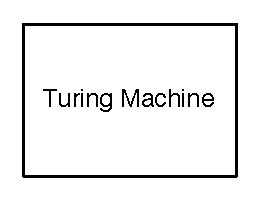
\includegraphics[width=0.8\textwidth]{block}
    \column{.45\textwidth}
Introduce the problem you are trying to solve,
motivate why solving this problem is important, highlight the
significance of solving this problem. (What are you trying to do and
why?)
\end{columns}
\end{frame}

\note{Notes can help you to remember important information. Turn on the notes option.}

\begin{frame}[c]{Proposed solution}
    \begin{figure}
        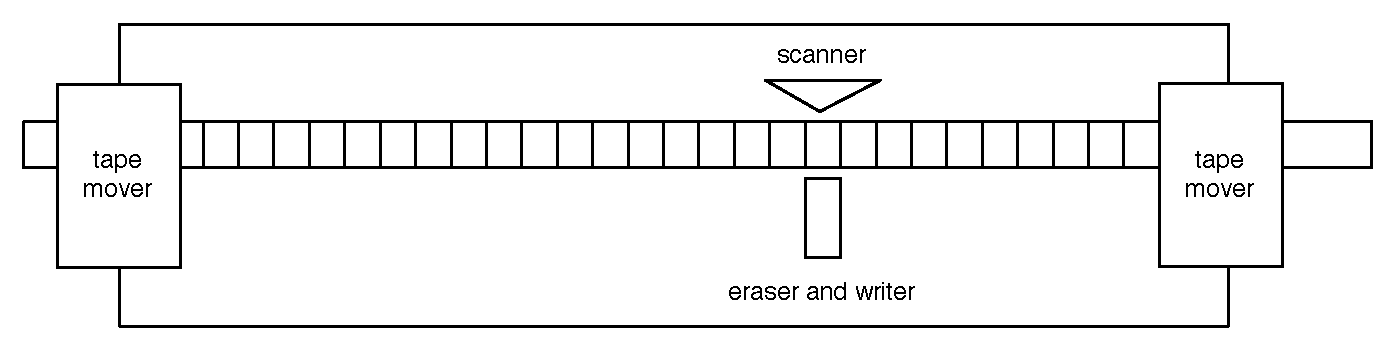
\includegraphics[width=0.8\textwidth]{turingmachine}
        \caption{How do you plan to solve this problem? Will you
require any hardware to do so (e.g., Raspberry Pies)? Will you require
any third-party software or libraries?}
    \end{figure}
\end{frame}

\note{Notes can help you to remember important information. Turn on the notes option.}

\begin{frame}[c]{Preliminary Time Plan}
\begin{theorem}
Provide a preliminary time plan (e.g., Gantt
chart in a readable form) and division of work among group members.
\end{theorem}
\end{frame}

\note{Notes can help you to remember important information. Turn on the notes option.}

\section{Section 2}

\begin{frame}[t]{Items and Numbers}
\begin{columns}
    \column{.5\textwidth}
            \begin{itemize}
            \item one
            \item two
            \item three
            \end{itemize}
    \column{.5\textwidth}
            \begin{enumerate}
            \item first
            \item second
            \item third
            \end{enumerate}
\end{columns}
\end{frame}


\begin{frame}[t,plain]
\lastpage{{\usebeamerfont{title} Questions?}\\[5ex]
author@email.com}
\end{frame}

\end{document}

